\documentclass[border=10pt]{standalone}
\usepackage{pgfplots}
\pgfplotsset{compat=1.18}
\begin{document}
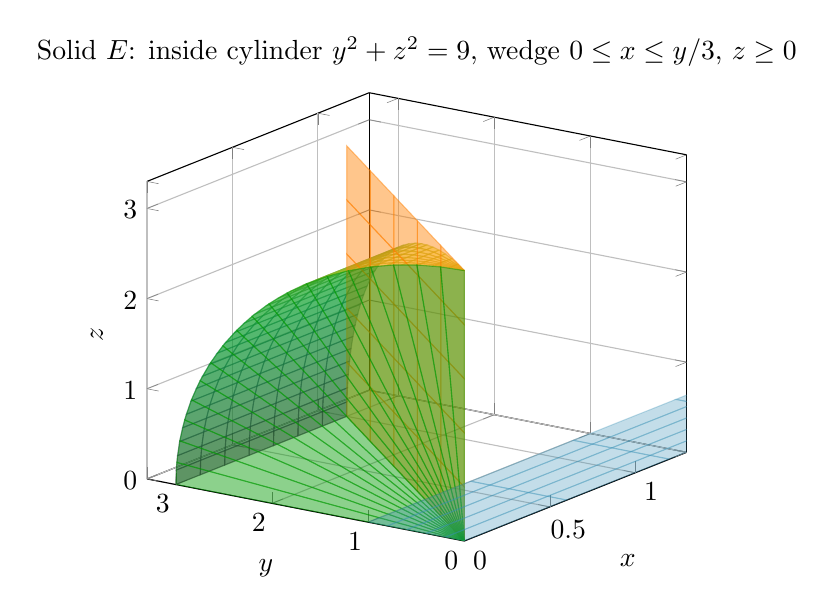
\begin{tikzpicture}
\begin{axis}[
    view={-55}{20},
    xlabel={$x$}, ylabel={$y$}, zlabel={$z$},
    xmin=0, xmax=1.3, ymin=0, ymax=3.3, zmin=0, zmax=3.3,
    grid=major,
    title={Solid $E$: inside cylinder $y^2+z^2=9$, wedge $0\le x\le y/3$, $z\ge0$},
]
% Cylinder surface y^2+z^2=9: u in [0,1] gives x = u*cos(v), v in [0,90] deg
\addplot3[surf, shader=faceted, opacity=0.45, colormap/viridis,
    domain=0:1, samples=8, y domain=0:90, samples y=30]
({x*cos(y)}, {3*cos(y)}, {3*sin(y)});
% Slanted plane x = y/3: x = u, y = 3u, z = w
\addplot3[surf, shader=flat, opacity=0.45, color=orange,
    domain=0:1, samples=6, y domain=0:3, samples y=6]
(x, {3*x}, y);
% Back face x=0: quarter disk in yz-plane
\addplot3[surf, shader=flat, opacity=0.45, color=green!60!black,
    domain=0:90, samples=20, y domain=0:1, samples y=2]
(0, {y*3*cos(x)}, {y*3*sin(x)});
% Bottom face z=0
\addplot3[surf, shader=flat, opacity=0.3, color=cyan!70!black,
    domain=0:1, samples=6, y domain=0:3, samples y=6]
(y, x, 0);
\end{axis}
\end{tikzpicture}
\end{document}